\documentclass[12pt]{article}

\usepackage{natbib}
\usepackage{amssymb}
\usepackage{amsmath}
\usepackage{bm}
\usepackage{dsfont}
\usepackage[margin=1in]{geometry}
\usepackage[font=scriptsize]{caption}
\usepackage{dsfont}
\usepackage{amsmath}
\usepackage{graphicx}
\usepackage{bm}
\newcommand{\m}[1]{\mathbf{\bm{#1}}}
\newcommand{\R}{I\hspace{-4.4pt}R}
\newcommand{\bc}[1]{\textcolor{blue}{\mathbf{#1}}}
\newcommand{\ind}{\mathds{1}}

% \setlength\parindent{0pt}

\makeatletter
\setlength{\@fptop}{0pt}
\makeatother


\begin{document}

\begin{Large}
\noindent \textbf{Extreme value comparison of CanCM4 simulations and observations}
\end{Large}
\bigskip

%\begin{large}
\noindent \textbf{Mickey Warner}
%end{large}


\section{Abstract}
\label{abstract}
We fit a Bayesian hierarchical model to threshold exceedances from CanCM4 climate simulations. Three simulation classes are analyzed: decadal, historical, and pre-industrial control. These are compared against on observation product. We find that in some domains, the simulations are in agreement with the observations, but in others can be quite different.

\section{Introduction}
\label{intro}

The Fourth Generation Coupled Global Climate Model (CanCM4) produces a wide array of atmospheric conditions across the globe. Two variables will be analyzed: precipitation (labled \texttt{pr}, in meters) and maximum temperature (labeled \texttt{tasmax}, in Kelvin). Three experimental classes that are of particular interest are decadal, historical, and pre-industrial control runs.

The decadal simulations provide climate estimates for ten years into the future, after conditioning on weather conditions at the time. We consider two decades in this analysis: 1962--1971 and 1990--1999, which are conditioned on climate states in 1961 and 1989, respectively. Historical simulations are obtained for the years 1961--2005 and are noted for including events that affect the climate such as volcanoes. The pre-industrial control, or simply control, simulations begin at climate conditions comparable to those preceding the industrial revolution and are run over a thousand years into the future. Decadal and historical simulations are run at $R=10$ different input settings. To obtain $R=10$ ``replicates'' for the control simulations, we randomly select ten non-overlapping 10-year periods.

% TODO: Talk about the grids, degree spacing or km

An observation product is obtained from \cite{maurer2002long}. The observations are based on daily measurements from weather stations throughout the United States and are interpolated onto a fine grid. To make the observations comparable to the climate simulations, we take weighted sums or averages of the climate simulations and just sums or averages of the observations. See section \ref{process} for details, along with other changes made to the data in preparation for analysis.

Being a threshold exceedance analysis, we must concern ourselves with exceedances occuring together within a short time. This is handled by studying the extremal index $\theta$, a measure of dependence among the extremes. With an estimate for $\theta$, we can ``decluster'' the exceedances to obtain independent clusters. The method for estimating $\theta$ and declustering has been generalized to the hierarchical setting, see section \ref{index}.

Having replicates of a time-series suggests the use of a hierarchical model, described in detail in section \ref{hier}. Under such a framework we can model each series separately, while assuming these series come from a larger population. In the analysis, we will place focus on the mean of this larger population, being akin to the ensemble average in a climate study.

The main focus of this paper is to compare the extreme values of the observation product with those of CanCM4 climate simulations. The comparison is done mostly through visualization of the differences between posterior parameters and a useful quantity called the return level (section \ref{return}).
% TODO: change this last sentence to talk about Bhatta dist



\section{Data pre-processing}
\label{process}

\subsection{Aggregation}
\label{aggregate}

\begin{figure}
\begin{center}
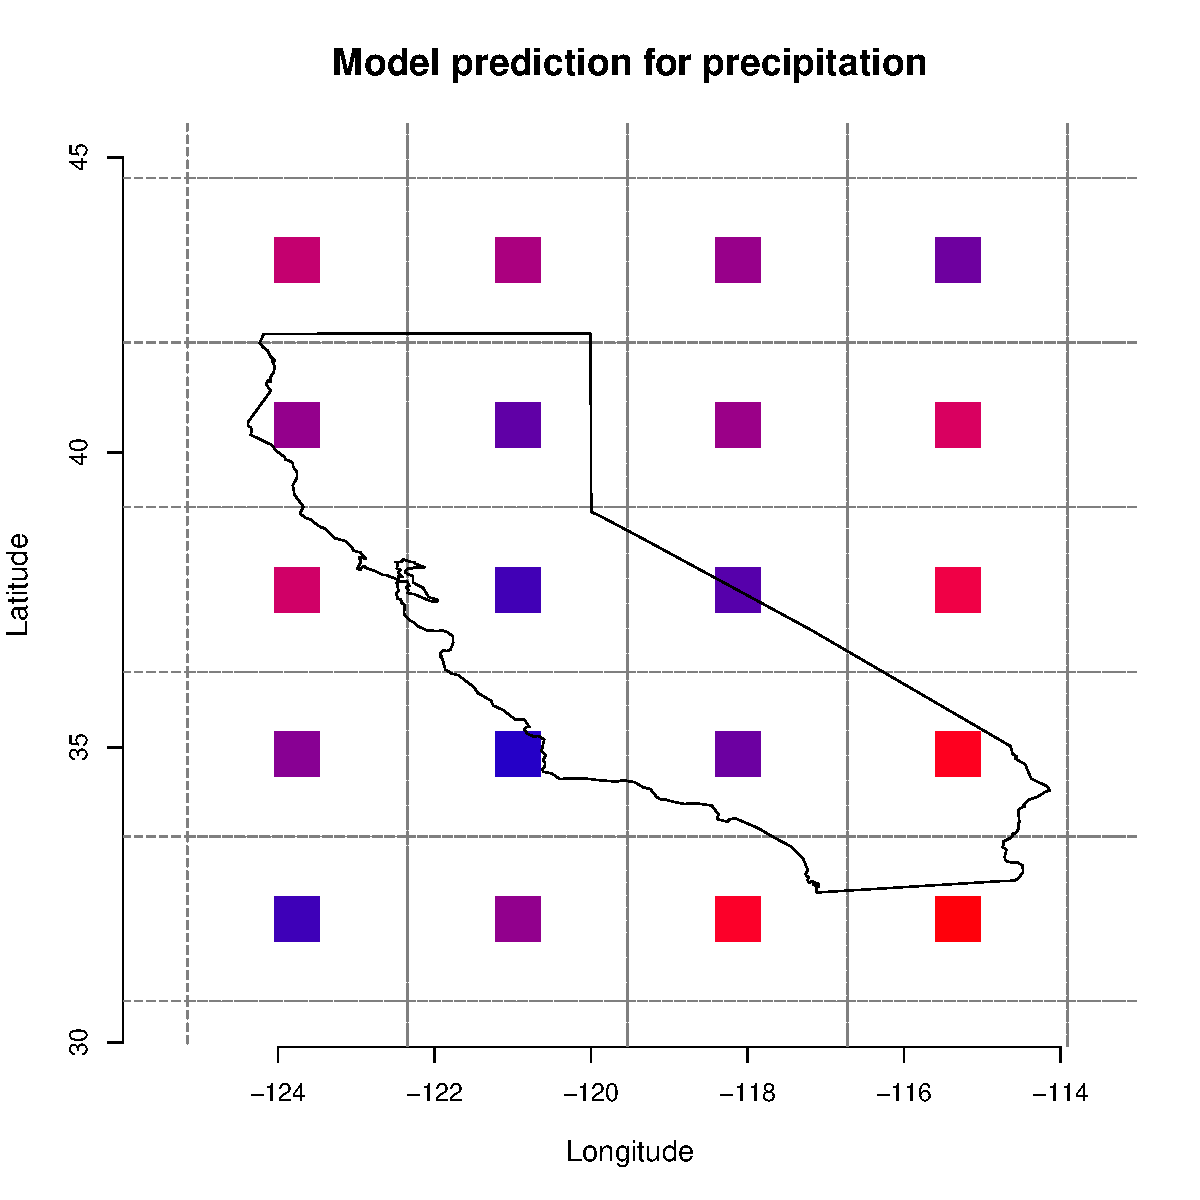
\includegraphics[scale=0.26]{figs/cal_mod_box1.pdf}
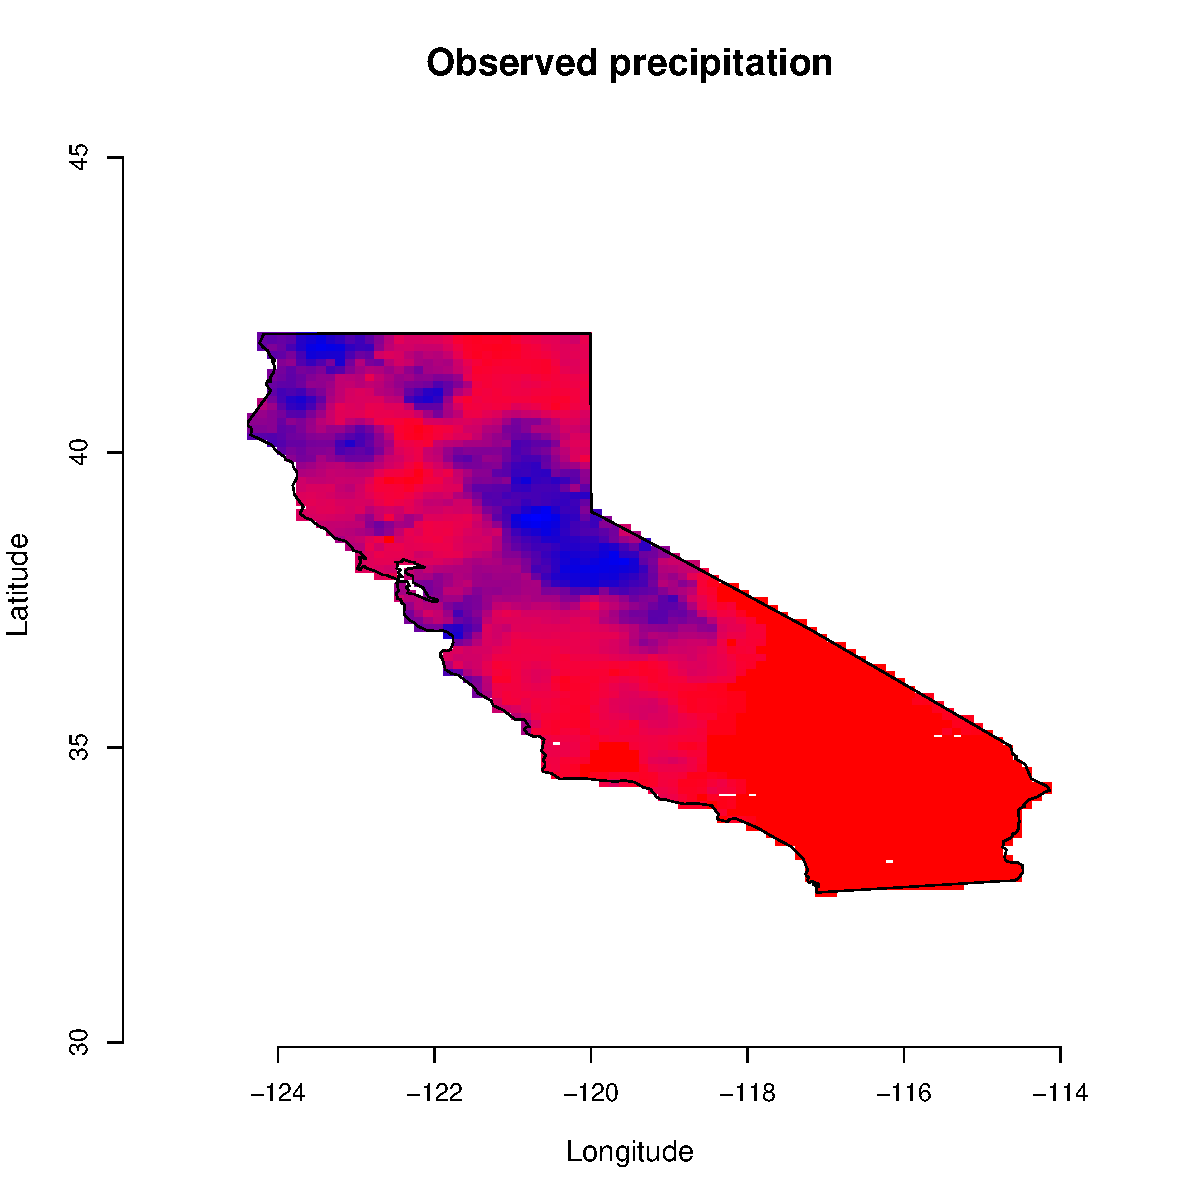
\includegraphics[scale=0.26]{figs/cal_mod_box2.pdf}
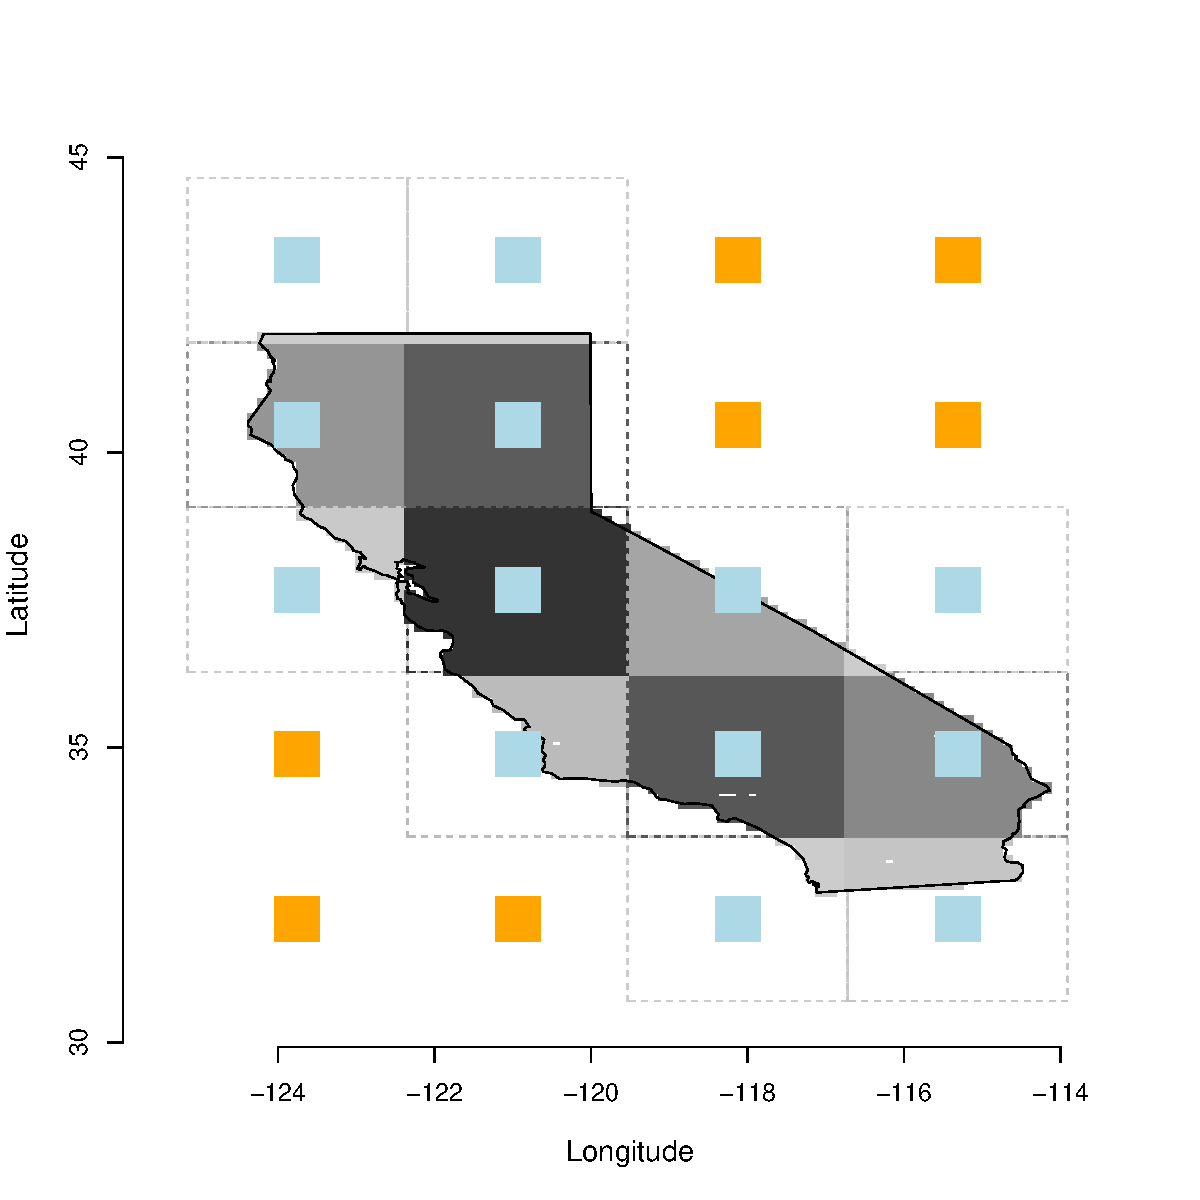
\includegraphics[scale=0.26]{figs/cal_mod_box3.pdf}
\end{center}
\caption{Left: CanCM4 simulation locations. Center: Observation locations. Right: method for computing weighted sum or average for CanCM4 to make values comparable with observations; the lighter gray points mean less weight is applied to the climate simulations and the darker gray means more weight. The data shown are from a single day in January.}
\label{weight}
\end{figure}

In this subsection, we describe how the simulations and observations were made to be comparable. Figure \ref{weight} shows the spatial locations of each data source. The plots show only California, but the climate simulations were over the entire globe and the observation product over the United States.

We will analyze precipitation and temperature over both California and the United States. In each case, we take the climate locations and create non-overlapping cells, or rectangles, such that each location is roughly in the center of the cell. Then we count the number of locations from the observation product that are contained with each cell. The number of locations within the cells are used to weight the climate simulations (the right-most plot in Figure \ref{weight} shows which climate simulation locations have non-zero weight). For precipitation, we take a weighted sum and for temperature a weight average. No weighting is used for the observations. Instead, a straight sum or average of all locations within our region of interest (either California or U.S.) is used. This method places the simulations and the observations on the same scale and yields time-series on daily time scales.

\subsection{De-trending}
\label{anomaly}

\begin{figure}
\begin{center}
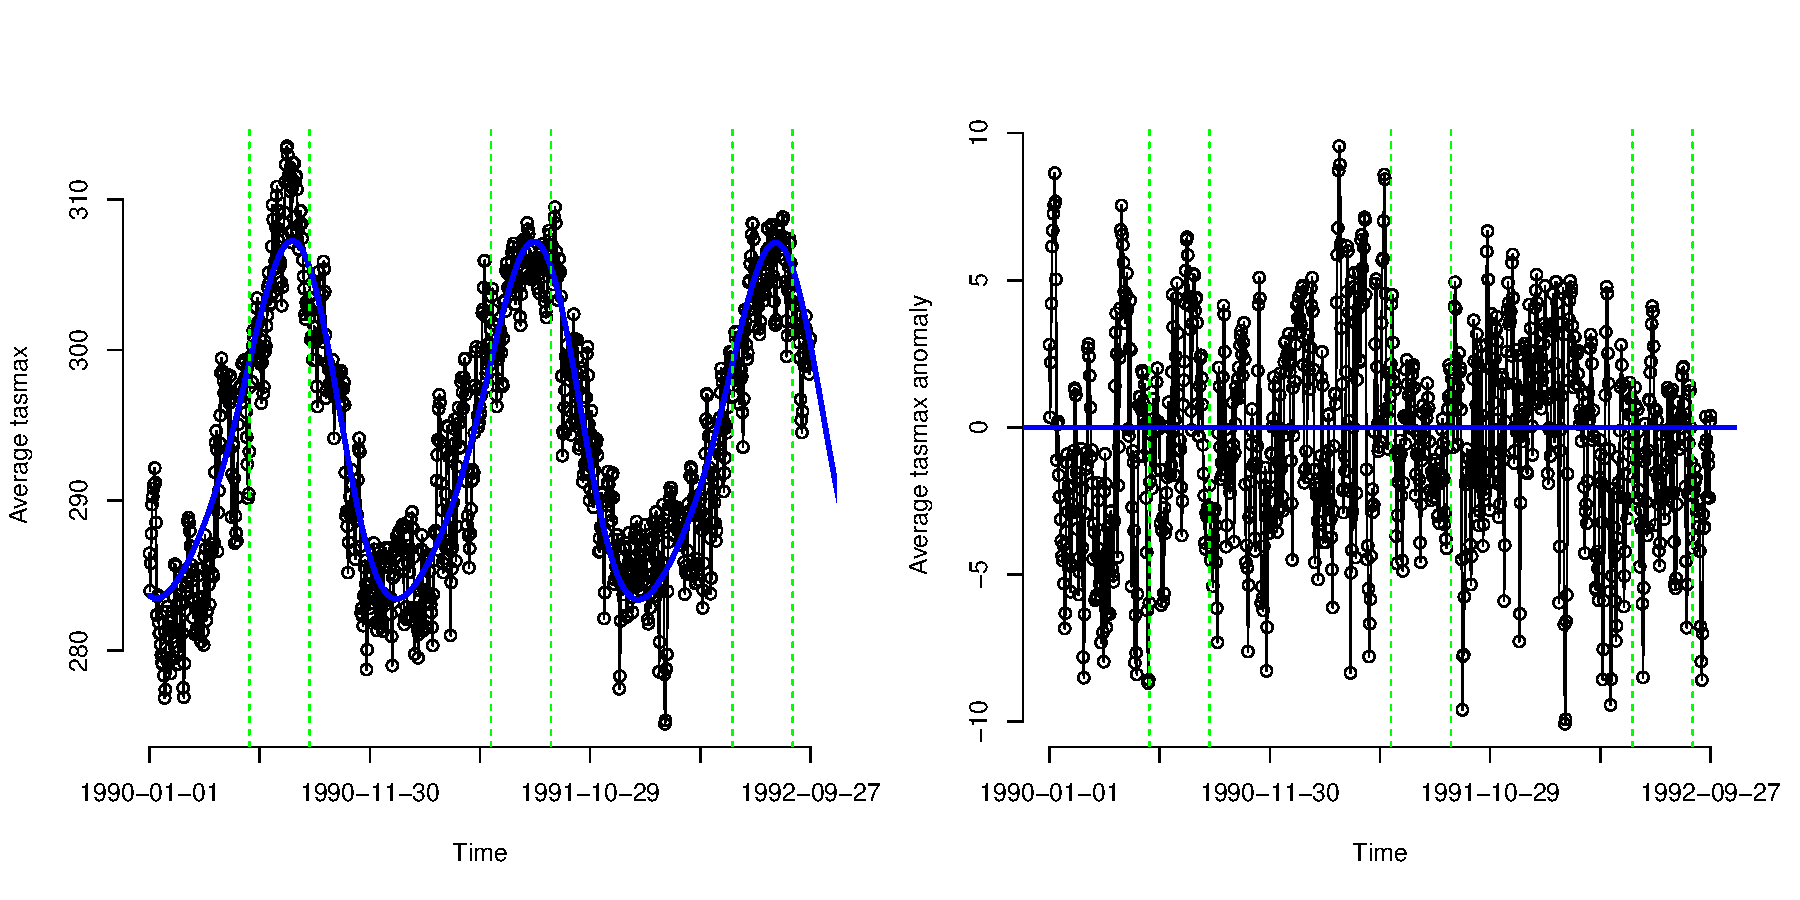
\includegraphics[scale=0.50]{figs/dlm.pdf}
\end{center}
\caption{One of the DLMs used to calculate the anomalies. Shown is one of the decadal replicates of average \texttt{tasmax} in California for about the first two and one-half years of the time-series. The green dashed lines mark the beginning and the end of the summer months.}
\label{dlm_fig}
\end{figure}

Each time-series is ``de-trended'' prior to declustering and parameter estimation. This is accomplished through the use of dynamic linear models (DLMs). We will review some basic concepts for DLMs, see \cite{prado2010time} chapter 4 for more details.

A normal DLM is specified by the quadruple $\{\m{F}_t, v_t, \m{G}_t, \m{W}_t\}$ which determine how a univariate time series $y_1,\ldots,y_T$ is modeled over time. We assume
\begin{align}
y_t &= \m{F}_t^\top\m{\theta}_t + \nu_t,~~~~~\nu_t\sim N(0, v_t) \label{dlm_model} \\
\m{\theta}_t &= \m{G}_t\m{\theta}_{t-1}+\m{w}_t~~~~~\m{w}_t\sim N(\m{0}, \m{W}_t) \nonumber
\end{align}
where $\m{\theta}_t$ is the length $p$ state vector, $\m{F}_t$ is a length $p$ vector of known constants are regressors, $\nu_t$ is obersvation noise, $\m{G}_t$ is the known $p\times p$ state evolution matrix, and $\m{w}_t$ is the state evolution noise. Note that $\nu_s$ and $\m{w}_t$ are independent and mutually independent.

An advantage to model (\ref{dlm_model}) is its capability in yielding a smooth and flexible mean across time. After conditioning on the data up to time $T$, we extrapolate back over time to obtain the posterior distributions $p(\m{\theta}_t|D_T)$ for all $t<T$, which have mean $\m{a}_t$. Using these distributions, and given $\m{F}_t$, the mean of $y_t$ is simply $\m{F}_t^\top\m{a}_t$ (we refer the reader to \cite{prado2010time} for the algorithmic details).

We must omit further details in the interest of space. Our DLM is finalized in the following way. We construct $\m{F}_t$ and $\m{G}_t$ such that the evolution of $\m{\theta}_t$ has annual and semi-annual periods, i.e. the first and second harmonics. Higher harmonics did not seem to make significant contributions in modeling the time-series. A discount factor of $\delta=0.9999$ was chosen, signifying low systematic variance. We assume the prior for $v_t$ is an inverse gamma having sensible shape and scale parameters.

In the end, we are left with what is shown in Figure \ref{dlm_fig}. The blue line in the left plot is the mean of $y_t$, $\m{F}_t^\top\m{a}_t$, given the whole time series. The interior of the vertical green lines mark the summer months. The right plot is the result of subtracting the observation $y_t$ with the mean from the DLM, which produces a roughly stationary sequence. Thus, in our extreme value analysis we work in the anomaly space.

For each time-series to be analyzed, we fit a DLM having the characteristics described above to obtain the anomalies. When working within a specific season, either winter (December, January, February) or summer (June, July, August), we extract just those days contained in the season and treat the beginning of a season as the day that follows immediately after the last day. So, for example in winter, 28 February is followed immediately by 1 December.


\section{Methods}

\subsection{Extremal Index}
\label{index}

% Sloppy, may not be technically correct with regard to theta.
The threshold exceedance model described in section \ref{thresh} relies on an assumption of independence which is unrealistic for a time-series. When there is dependence between the random variables, the extremes are related according to the so-called extremal index, denoted by $\theta\in(0,1]$. The extremal index can loosely be interpreted as
\[ \theta = (\mathrm{limiting~mean~cluster~size})^{-1}. \]
As an example, suppose $\theta=0.5$, then we would expect exceedances of a large threshold to occur in pairs; for $\theta=0.33$, in groups of 3.

\cite{ferro2003inference} show that the extremal index arises in the limiting distribution of the times between exceedances of a threshold. If $T_\theta$ is the random variable for interexceedance times in the limit, then $T_\theta$ is distributed according to the mixture
\begin{align}
(1-\theta)\epsilon_0 + \theta \mu_\theta
\end{align}
where $\epsilon_0$ is the degenerate probability distribution at $0$ and $\mu_\theta$ is an exponential distribution with mean $\theta^{-1}$. This means that the role of $\theta$ is two-fold: it is both the proportion of non-zero interexceedance times and the inverse mean of non-zero interexceedance times. This poses a challenge when estimating $\theta$ since is it impossible to observe an interexceedance time of zero in practice.

We next describe the hierarchical model used to esimate $\theta$. This is distinct from the threshold exceedance model and is used only in getting a single estimate for $\theta$, which is used to decluster the exceedances and to calculate return levels.

\subsubsection{Estimation}

\cite{ferro2003inference} propose estimating $\theta$ by considering the interexceedance times, the length of time between each random variable that exceeds the threshold. Suppose we have observations $X_1,\ldots,X_n$. For a threshold $u$, the $N$ exceedances $Y_i=X_i-u$ given $X_i>u$ occur at times $1\leq j_1<\cdots< j_N\leq n$. The observed interexceedance times are given by $T_i=j_{i+1}-j_i$ for $i=1,\ldots,N-1$. The following log-likelihood is then provided
\begin{align}
l(\theta, p; \m{T}) =& m_1\log(1-\theta p^\theta) + (N-1-m_1)\{\log(\theta)+ \log(1-p^\theta)\} \nonumber \\
 &+ \theta\log(p)\sum_{i=1}^{N-1}(T_i-1) \label{ferro}
\end{align}
where $p$ is the probability of not exceeding the threshold. We require this likelihood to be used in a hierarchical model.

Suppose we have $R$ replicates from a climate model with values from replicate $i$ denoted $X_{i,1},\ldots,X_{i,n}$. If we assume these simulations are independent from each other, then we expect there to be $R$ unique extremal indices $\theta_1,\ldots,\theta_R$. However, since these all come from the same climate model, we may wish to assume that the $\theta_i$ come from a common distribution,
\[ \theta_i \overset{iid}\sim Beta\left(\theta\nu, (1-\theta)\nu\right). \]
Under model (\ref{ferro}), we place a similar prior on the $p_i$,
\[ p_i \overset{iid}\sim Beta\left(p\tau, (1-p)\tau\right). \]

The model is completed by choosing priors for $\theta$, $\nu$, $p$, and $\tau$---the latter two parameters being required only for model (\ref{ferro}). We assume
\begin{align*}
\theta &\sim Beta(a_\theta, b_\theta) \\
\nu &\sim Gamma(a_\nu, b_\nu) \\
p &\sim Beta(a_p, b_p) \\
\tau &\sim Gamma(a_\tau, b_\tau) 
\end{align*}
with the hyperparameters chosen to be
%\begin{table}[h]
\begin{center}
\begin{tabular}{rlcl}
$\theta$: & $a_\theta = 1          $ &~~& $b_\theta = 1/2             $ \\
$   \nu$: & $   a_\nu = 1          $ &~~& $   b_\nu = 1/10            $ \\
$     p$: & $     a_p = 100 \hat{F}$ &~~& $     b_p = 100 (1-\hat{F}) $ \\
$  \tau$: & $  a_\tau = 1          $ &~~& $  b_\tau = 1/10            $ \\
\end{tabular}
\end{center}
%\end{table}
where $\hat{F}=\sum_{i=1}^R\sum_{j=1}^n \ind(X_{i,j}\leq u)$. Our parametrization for the gamma random variables are such that $X\sim Gamma(\alpha,\beta)$ has mean $\alpha/\beta$. The prior values for $\theta$ attempt to mitigate some of the issues surrounding model (\ref{ferro})

By assuming indepedence between the simulations, we can construct the following log-likelihood
\begin{align}
L = \sum_{i=1}^R l(\theta_i, p_i; \m{T}^{(i)}) \label{hiertheta}
\end{align}
where $\m{T}^{(i)}$ is the vector of interexceedance times for replicate $i$ having length $N_i$. In this univariate setting for the observation product, only model (\ref{ferro}) is needed.

\cite{suveges2007likelihood} proposed on an alternative likelihood for estimating the extremal index which dealt with some of the issues noted in \cite{ferro2003inference}. This likelihood was extended in \cite{suveges2010model}. Though there are advantages to the alternative likelihood, we prefer to use that given in (\ref{ferro}). In a separate simulation study, both likelihoods performed very similarly, with some preference to model (\ref{ferro}) within the hierarchical setting.

\subsubsection{Declustering}

Declustering is done as given in \cite{ferro2003inference}. Each replicate is declustered separately. Let $\hat{\theta_i}$ be the posterior mean of the extremal index of each replicate. Calculate $C_i=\lfloor \hat{\theta_i} N_i \rfloor + 1$, the estimated number of independent clusters. Let $T_{C_i}$ be the $C_i$th largest interexceedance time in $\m{T}^{(i)}$. In the case of ties, decrement $C_i$ by one until $T_{C_i+1}$ is strictly greater than $T_{C_i}$. Clusters are formed by grouping the exceedances that are separated in time by no more than $T_{C_i}$. In other words, two exceedances are in the same cluster if their interexceedance time is less than or equal to $T_{C_i}$.

The $C_i$ clusters that will be formed using the above scheme are assumed to be independent. For each cluster we compute the cluster maximum, this being the ultimate quantity used in our inference.



\subsection{Threshold exceedance model}
\label{thresh}

\subsubsection{Univariate}
\label{univariate}

Under some mild assumptions, for random variable $X$ and for large enough $u$, the distribution of $X-u$ (the exceedance), conditional on $X>u$ is approximately
\begin{align}
P(X-u\leq y|X>u) \approx H(y) = 1 - \left(1+\frac{\xi y}{\sigma}\right)^{-1/\xi} \label{gpapprox}
\end{align}
defined on $\{y:y>0~\mathrm{and}~(1+\xi y/\sigma) >0\}$. $H(y)$ is the distribution function for a generalized Pareto random variable with shape paremeter $\xi\in\R$ and scale $\sigma>0$.

Let $X_1,\ldots,X_n$ be a sequence of i.i.d. random variables and $u$ be a high threshold. Define $Y_i=X_i-u$ for $X_i>u$ be the $k$ exceedances. The likelihood of $(\xi,\sigma)$ is derived from (\ref{gpapprox}) as
\begin{align}
L(y_1,\ldots,y_k;\sigma,\xi)=\sigma^{-k}\sum_{i=1}^k\left(1+\frac{\xi y_i}{\sigma}\right)_+^{-1/\xi-1} \label{gplike}
\end{align}
where $z_+=\max(z,0)$. This provides the basis for an extreme value analysis. For example, after declustering, the cluster maxima (which are roughly independent) may be fit using likelihood (\ref{gplike}).

\subsubsection{Hierarchical model}
\label{hier}

Suppose we have $R$ replicates or computer simulations, each with $n_i$ observations, for $i=1,\ldots,R$. Let $X_{ij}$ denote the $j$th observation in replicate $i$. We assume
\[ X_{ij} \sim F_i,~~~~~i=1,\ldots,R,~~~~~j=1,\ldots,n_i \]
and all $X_{ij}$ are mutually conditionally independent. From (\ref{gplike}), we deriv

For a fixed $u$ and each $i$, define the following sets:
\[ A_i = \{j:x_{ij}\leq u\},~~~ A_i^c = \{j: x_{ij}>u\} \]
where $|A_i|=n_i-k_i$ and $|A_i^c|=k_i$ with $k_i$ being the number of exceedances in replicate $i$. We define our exceedances as
\[ y_{ij} = (x_{ij}-u)\cdot \ind_{(j \in A_i^c)} \]
so that all observations not exceeding $u$ are marked as $0$. Let $\m{y}_i=(y_{i,1},\ldots,y_{i,n_i})^\top$ and $\m{y}=(\m{y}_1^\top,\ldots,\m{y}_R^\top)^\top$.

The likelihood is given by
\begin{align}
L(\m{y}; \m{\sigma}, \m{\xi}, \m{\zeta}) &= \prod_{i=1}^R f_{Y_i}(\m{y}_i|\sigma_i,\xi_i,\zeta_i) \nonumber \\
&= \prod_{i=1}^R\left[\prod_{j\in A_i} F_{X_i}(u) \times \prod_{j\in A_i^c} f_{X_i}(y_{ij}+u)\right] \nonumber \\
&\approx \prod_{i=1}^R\left[\prod_{j\in A_i} F_{X_i}(u) \times \prod_{j\in A_i^c} [1-F_{X_i}(u)]h(y_{ij}|\sigma_i,\xi_i)\right]~~~~~\mathrm{(approximation~(\ref{gpapprox}))} \nonumber \\
&= \prod_{i=1}^R\left[\prod_{j\in A_i} (1-\zeta_i)\times \prod_{j\in A_i^c} \frac{\zeta_i}{\sigma_i}\left(1+\xi_i\frac{y_{ij}}{\sigma_i}\right)_+^{-1/\xi_i-1}\right]~~~~~(\zeta_i=1-F_{X_i}(u)) \nonumber \\
&= \prod_{i=1}^R\left[(1-\zeta_i)^{n_i-k_i}\zeta_i^{k_i}\prod_{j\in A_i^c}\frac{1}{\sigma_i}\left(1+\xi_i\frac{y_{ij}}{\sigma_i}\right)_+^{-1/\xi_i-1}\right] \label{biglike}
\end{align}

Note that the parameters describing the tail of $F_i$ (i.e. $\xi_i,\sigma_i$) depend only on those observations which exceed $u$. The parameter $\zeta_i=P(X_{ij}>u)$, which is necessary for calculating return levels (section \ref{return}), is based only on the number of exceedances. This justifies the use of cluster maxima for $\m{y}_i$.

We complete the hierarchical model formulation by specifying the following priors:
\begin{align}
\xi_i|\xi, \tau^2  &\sim Normal(\xi, \tau^2) \nonumber \\
\sigma_i|\alpha, \beta &\sim Gamma(\alpha, \beta) \nonumber \\
\zeta_i|\zeta, \eta &\sim Beta(\zeta\eta, (1-\zeta)\eta) \nonumber \\
 \label{priors} \\
\xi &\sim Normal(m, s^2)&  &\tau^2 \sim Gamma(a_\tau, b_\tau) \nonumber \\
\alpha &\sim Gamma(a_\alpha, b_\alpha)&  &\beta \sim Gamma(a_\beta, b_\beta) \nonumber \\
\zeta &\sim Beta(a_\zeta, b_\zeta)&  &\eta \sim Gamma(a_\eta, b_\eta) \nonumber
\end{align}
By combining (\ref{biglike}) and (\ref{priors}) we obtain the full posterior distribution. Samples are obtained via MCMC.



\subsection{Return levels}
\label{return}

A most useful quantity in an extreme value analysis is the return level. Generally, for a distribution $G$, the return level $x_m$ is the solution to
\begin{align}
G(x_m) = 1-\frac{1}{m}
\end{align}
and has the convenient interpretation as the quantity that is exceeded on average once every $m$ observations.
% TODO: needs more intuition

When working with the generalized Pareto model (\ref{gpapprox}), it can be shown that the $m$-observation return level is
\begin{align}
x_m = u +\frac{\sigma}{\xi}\left[\left(m\zeta\theta\right)^\xi-1\right] \label{rl}
\end{align}
where the terms $\zeta$ and $\theta$ account for the probability of exceeding $u$ and being within a cluster, respectively. Using MCMC samples, we can obtain a distribution for $x_m$, but note that the posterior mean for $\theta$ is used, not samples obtained using (\ref{hiertheta}), when calculating the return level.


\subsection{Bhattacharyya distance}
\label{bhatta}

\cite{bhattacharyya1943measure} proposed a means for measuring the degree of similarity between two probability distributions. For two continuous random variables on support $\mathcal{X}$ with densities $p$ and $q$, the Bhattacharyya coefficient is defined as
\begin{align}
BC(p,q)=\int_\mathcal{X} \sqrt{p(x)q(x)} dx. \label{bhattacoef}
\end{align}
The Bhattacharyya distance is 
\begin{align}
D_B(p,q)=-\log BC(p,q).
\end{align}
We use kernel density estimation to calculate $p$ and $q$ along a grid of the support and then approximate the integral in (\ref{bhattacoef}). If the support is different for the two random variables (as will typically be the case when comparing random variables whose parameters determine the support such as the generalized Pareto), we will integrate over the intersection of the supports.

Since our focus is on comparing the climate model simulations with the observations, we will compare the posterior distributions of parameters or quantities (i.e. return level) with Bhattacharyya distance. The idea is to compute distances from the replicates to their mean and determine whether the observations could have reasonably come from the climate model.

Taking the shape parameter as an example, from the hierarchical model in \ref{hier} we have posterior samples for $\xi_1^c,\ldots,\xi_R^c$ for, say, some decadal simulations. We also have posterior samples for the mean $\xi^c$. Using the kernel density estimation mentioned earlier, we obtain $R$ Monte Carlo estimates $D_B(\xi_i^c, \xi^c)$, for $i=1,\ldots,R$. From the univariate model \ref{univariate} we have the shape parameter $\xi^o$ for the observation product. Finally, we calculate $D_B(\xi^o, \xi^c)$ and ask whether this quantity falls within the range of $D_B(\xi_i^c, \xi^c)$. When this occurs, we say $\xi^o$ is ``similar'' to the $\xi_i^c$ since the observation differs from the mean climate model in a similar way as the replicates differ from the mean.

\section{Results}
\label{results}

For each of the four data sources (i.e. the three climate simulation classes and the observation produce), there are four factors with two levels each. The factors, with their levels, are:
\begin{enumerate}
\item Variable --- precipitation or maximum temperature
\item Season --- winter or summer
\item Decade --- 1962--1971 or 1990--1999
\item Region --- California or U.S.A.
\end{enumerate}
There are then 16 combinations of the factors to be made. For each combination, the hierarchial model described in section \ref{hier} is fit to the decadal, historical, and control runs; the univariate model in section \ref{univariate} is fit to the observation product since this data source does not have replicates.

The next six figures shows posterior parameters and other quantities of interest. For the hierarchical model, we show the results of the \emph{mean} process. For example, in Figure \ref{ksi} the parameter shown is the posterior for $\xi$, the mean of $\xi_1,\ldots,\xi_R$. This is in opposition to inference on an unknown replicate which would require sampling, among other things, a new shape parameter $\xi^*$. Therefore, the intervals are more narrow than if we looked at the posterior predictive distribution for a new replicate, but the parameters will be comparable to those from the univariate model with the observations and give us a sense of how the climate simulation performs on average.

The posterior shape parameters in Figure \ref{ksi} show overlapping bounds in many cases, but in some combinations of factors we can seem some departure from the observations. The numbers shown above the lines are the thresholds: $0.95$ quantile for the climate simulations and $0.85$ for the observations. The quantity itself is not too important since different thresholds may produce similar return levels. Figure \ref{sigma} shows the logarithm of the mean scale parameter, $\log(\sigma)$ for the observations and $\log(\alpha/\beta)$ for the simulations.

Figures \ref{20rl} and \ref{50rl} give the $20$- and $50$-year return levels, respectively. In these figures, we have the same $x$-axes for the columns in total precipiation and for the columns under average maximum temperature. Some intervals are difficult to see given the scale, but we can still inspect how the return levels from the observations differ from those of the climate siulations. For winter precipitation, we see that the climate simulations underestimate the return level in california, but does much better when over the whole of the United States.

Figure \ref{tail} shows posterior predictive samples (based on the mean parameters for the hierarchical model) drawn from the generalized Pareto distribution, conditioned on the random variables being greater than the given threshold. There is significant overlap of the simulations with the observations, but this alone does not suggest accuracy of the simulations. Thus, the aforementinoed return levels are necessary when determining similarities and differences.

The posterior mean and 95\% highest posterior density intervals for the extremal index are shown in Figure \ref{theta}. The climate simulations seem to be consistent with the observations for the temperature, but not so for precipiation where they tend to overestimate $\theta$. Though, in terms of limiting mean cluster size, there is not a great difference between $1/0.5=2$ and $1/0.8=1.25$.

Recall that these results are based on the anomalies, the difference between the daily values and their average. Predictions based on the hierarchical and univariate models proposed in section \ref{thresh} can only be of practical use if the average is also given. This may be simple to calculate for the climate simulations, but more care would be needed for projecting the average of the observations. We have not considered this in our analysis.

\begin{figure}
\begin{center}
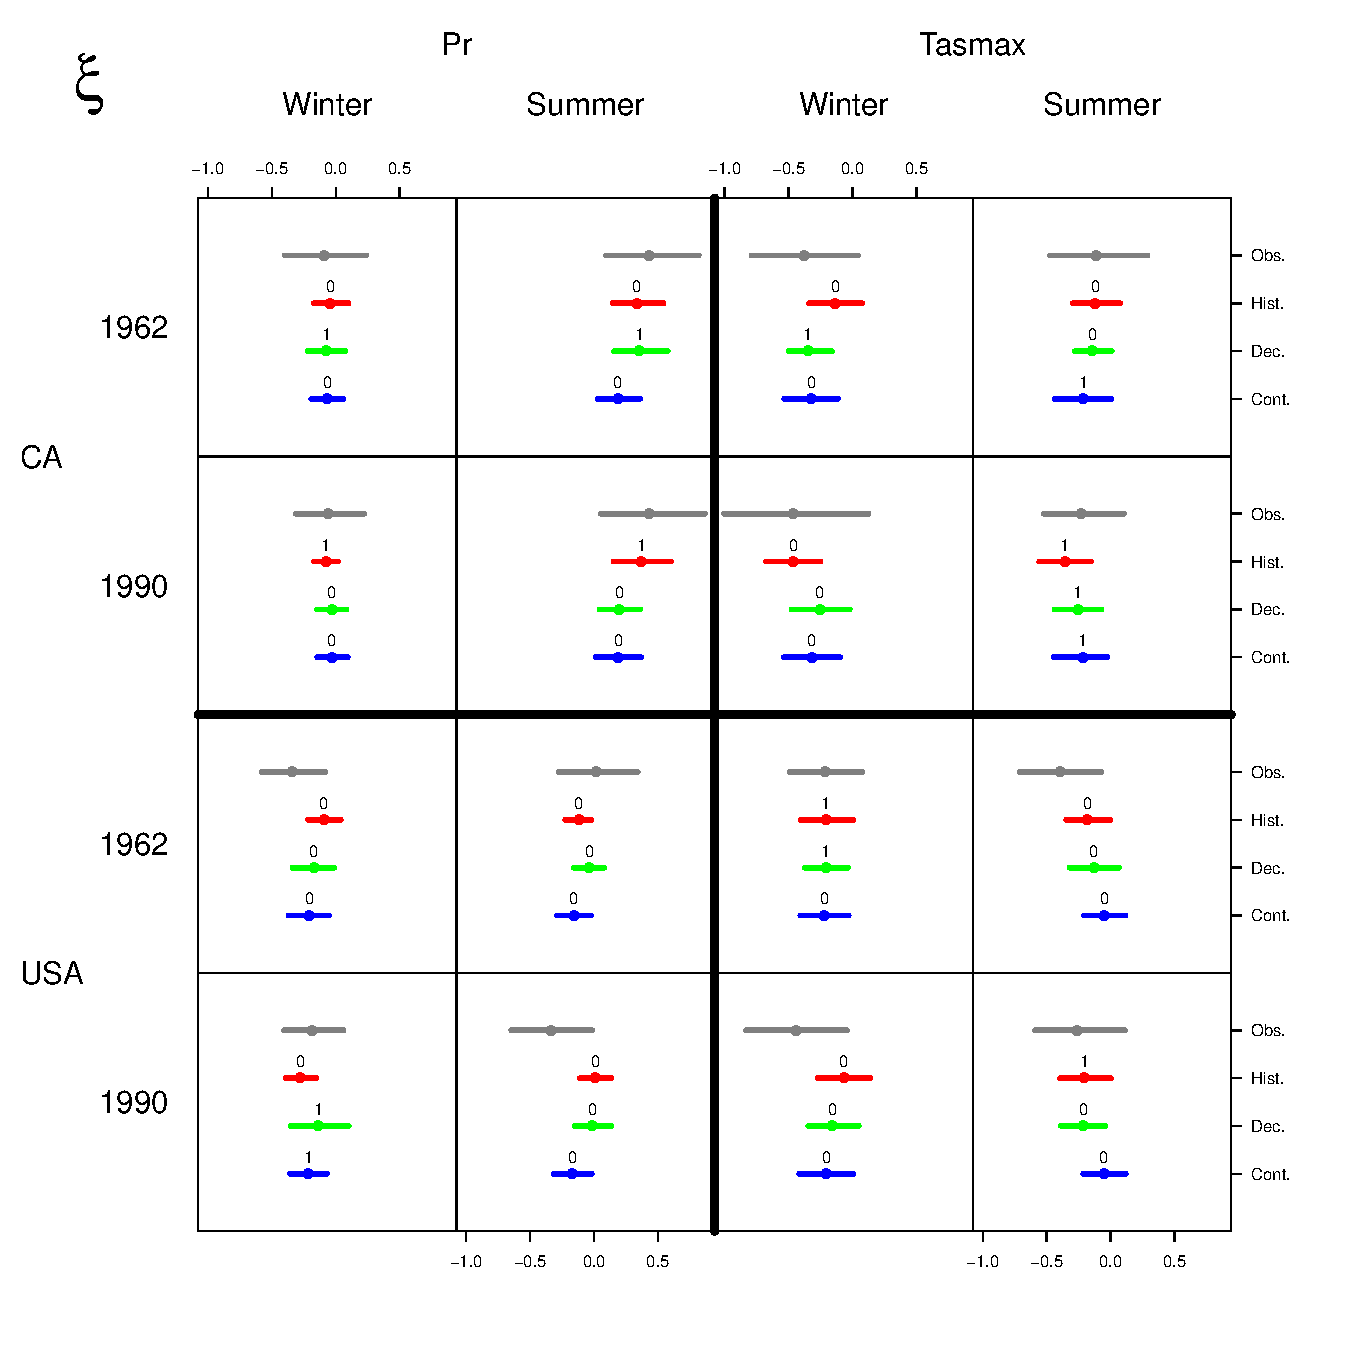
\includegraphics[scale=0.72]{figs/shape.pdf}
\end{center}
\caption{Posterior shape parameter, $\xi$, under each domain and each of the four data types. The points are the means and the lines mark the 95\% h.p.d. intervals. The number above each point marks whether the observations are similar (in the sense of Bhattacharyya distance) to the replicates of that climate model type---1 means similar, 0 mean not similar. Note: The $x$-axes are the same for every plot. The $y$-axes (for this and all subsequent figures) denote only the data type and thus hold no quantitative meaning.}
\label{ksi}
\end{figure}

\begin{figure}
\begin{center}
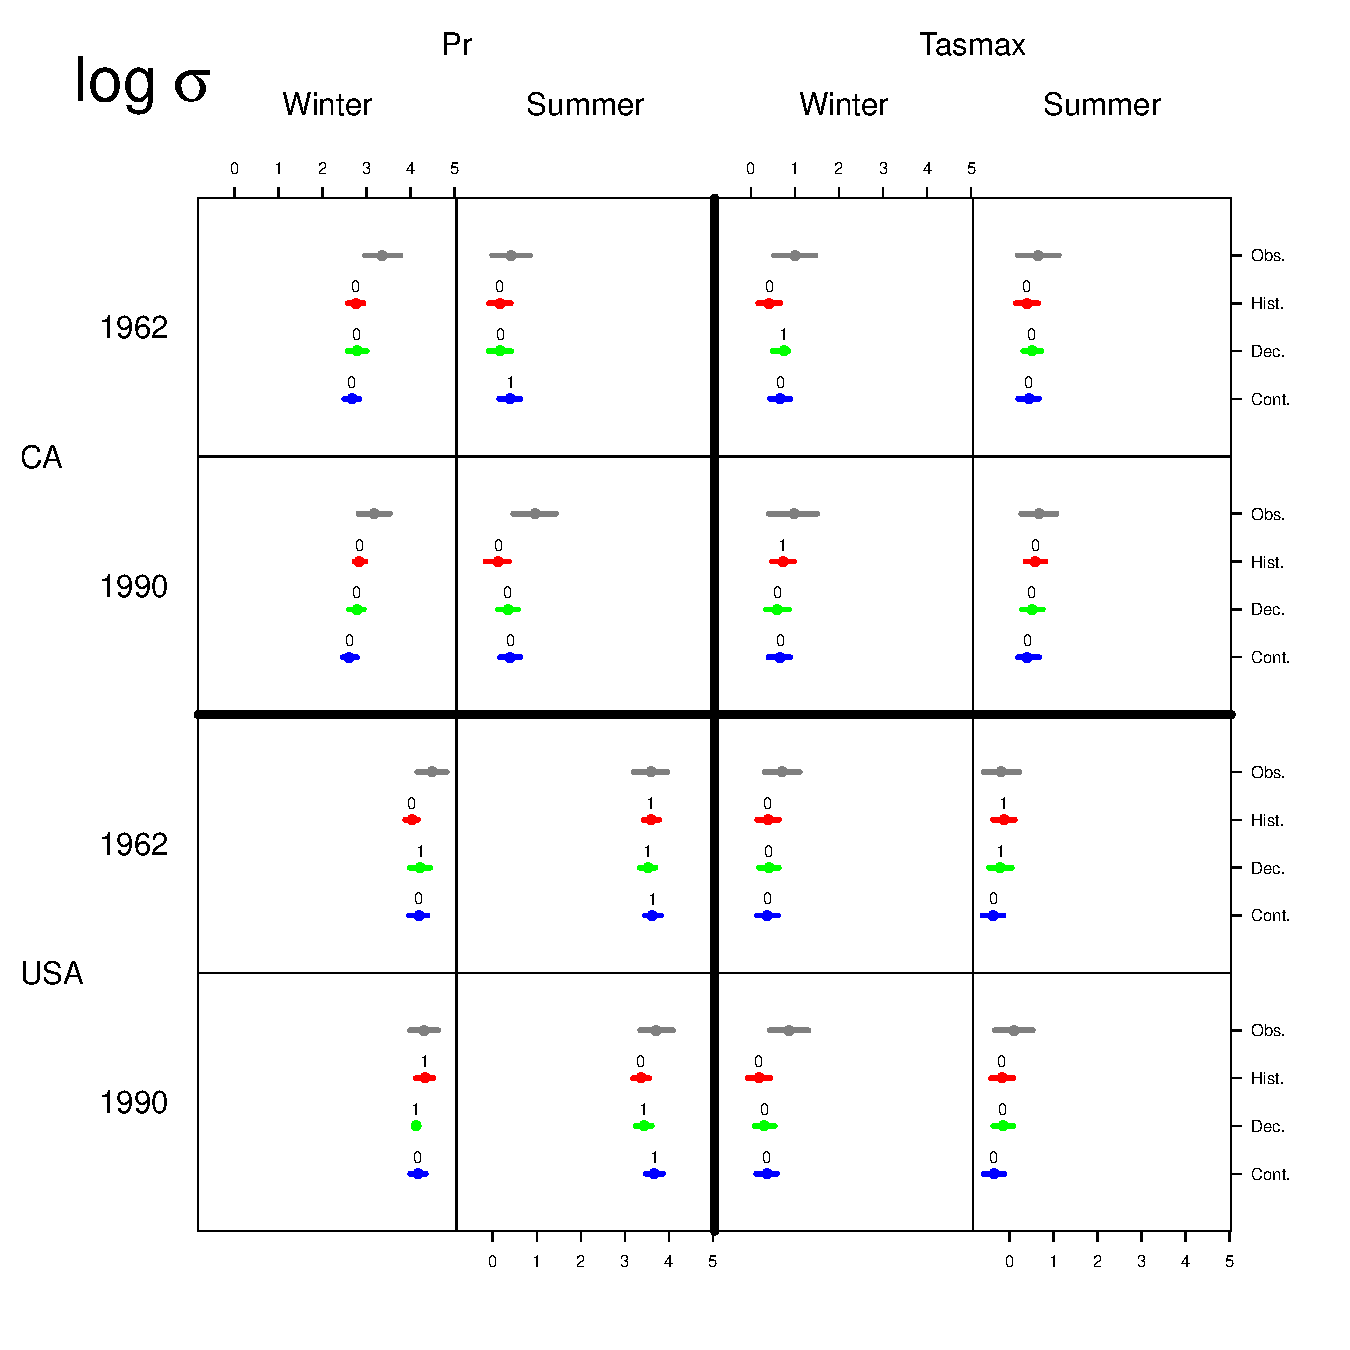
\includegraphics[scale=0.72]{figs/log_sigma.pdf}
\end{center}
\caption{Natural logarithm of the posterior scale. For the CanCM4 simulations, the parameter shown is $\log (\alpha/\beta)$ (the mean scale) because $\sigma_i$ follows a Gamma distribution with mean $\alpha/\beta$. No change of variables is necessary for the observations. Note: The $x$-axes are the same for every plot.}
\label{sigma}
\end{figure}

\begin{figure}
\begin{center}
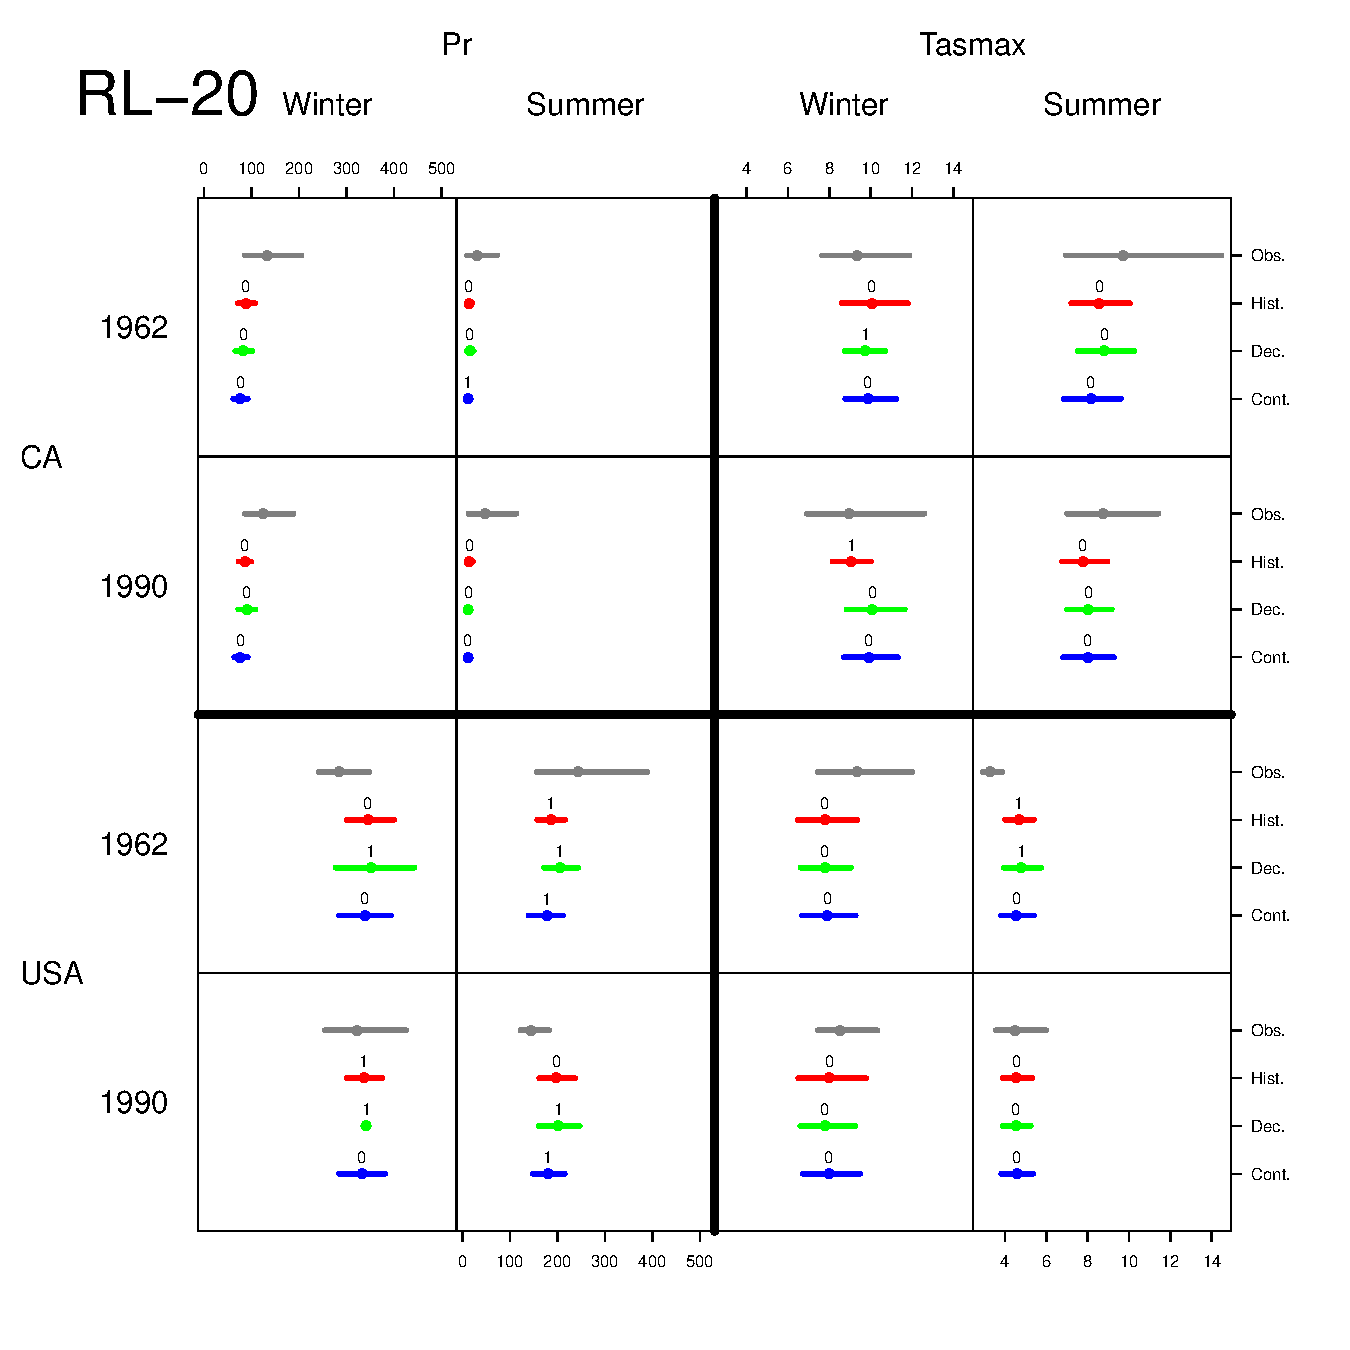
\includegraphics[scale=0.72]{figs/rl20.pdf}
\end{center}
\caption{20-year return levels. Note: The left two columns have the same $x$-axes, which are different than those in the right two columns, which have the same.}
\label{20rl}
\end{figure}

\begin{figure}
\begin{center}
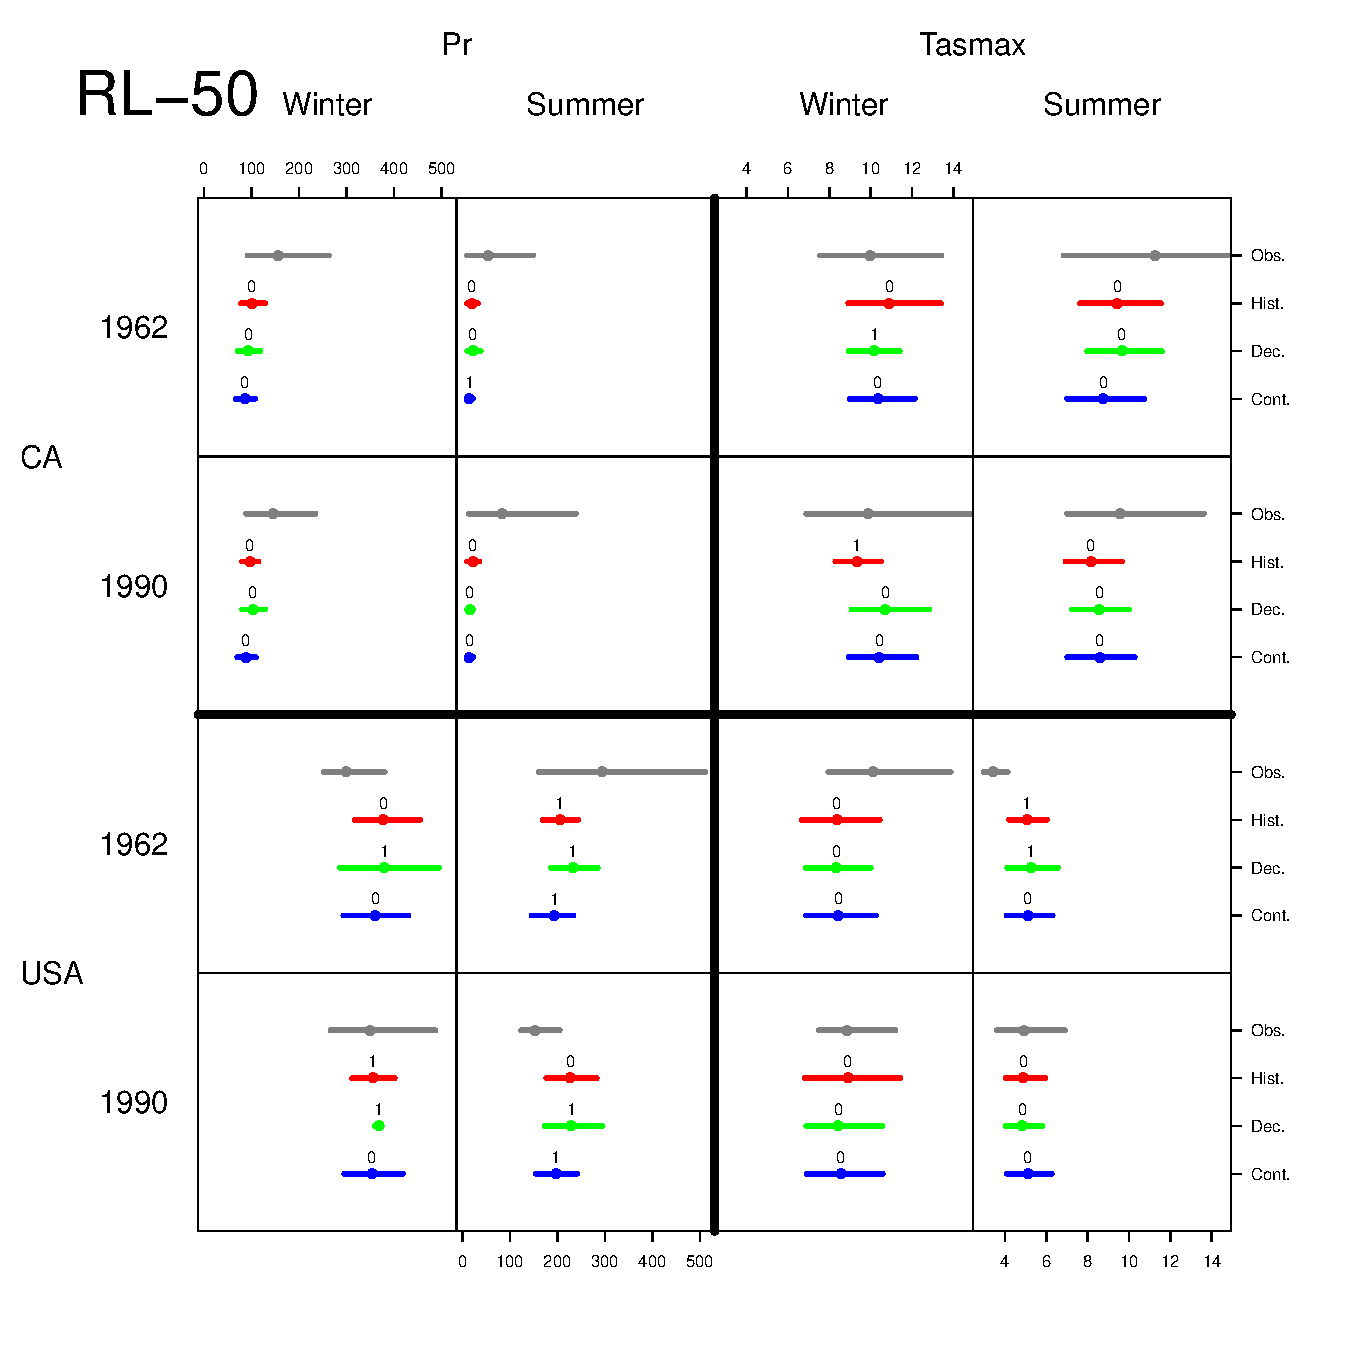
\includegraphics[scale=0.72]{figs/rl50.pdf}
\end{center}
\caption{50-year return levels. The $x$-axes are the same as those in Figure \ref{20rl}.}
\label{50rl}
\end{figure}

\begin{figure}
\begin{center}
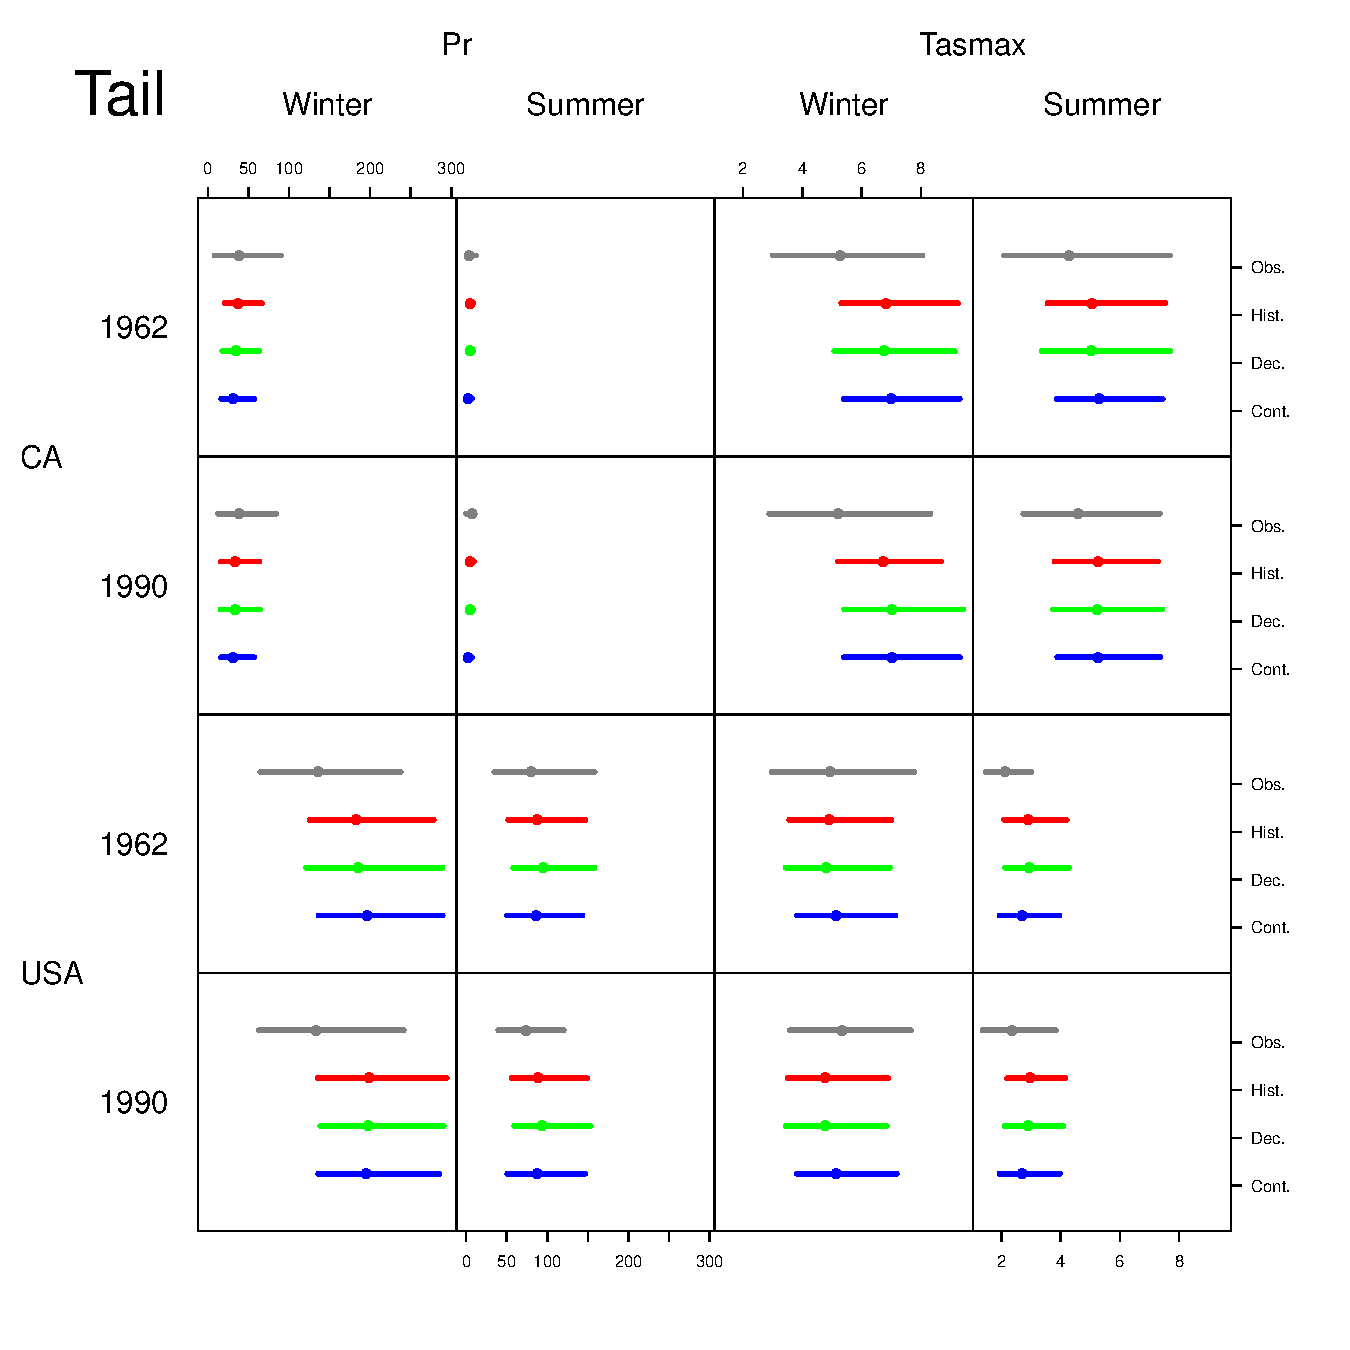
\includegraphics[scale=0.72]{figs/tail.pdf}
\end{center}
\caption{Mean and 95\% h.p.d. for the upper tail (i.e. the generalized Pareto) of the ensemble average. Similar to Figures \ref{20rl} and \ref{50rl}, the left two columns have the same $x$-axes and the right two columns have the same $x$-axes.}
\label{tail}
\end{figure}

\begin{figure}
\begin{center}
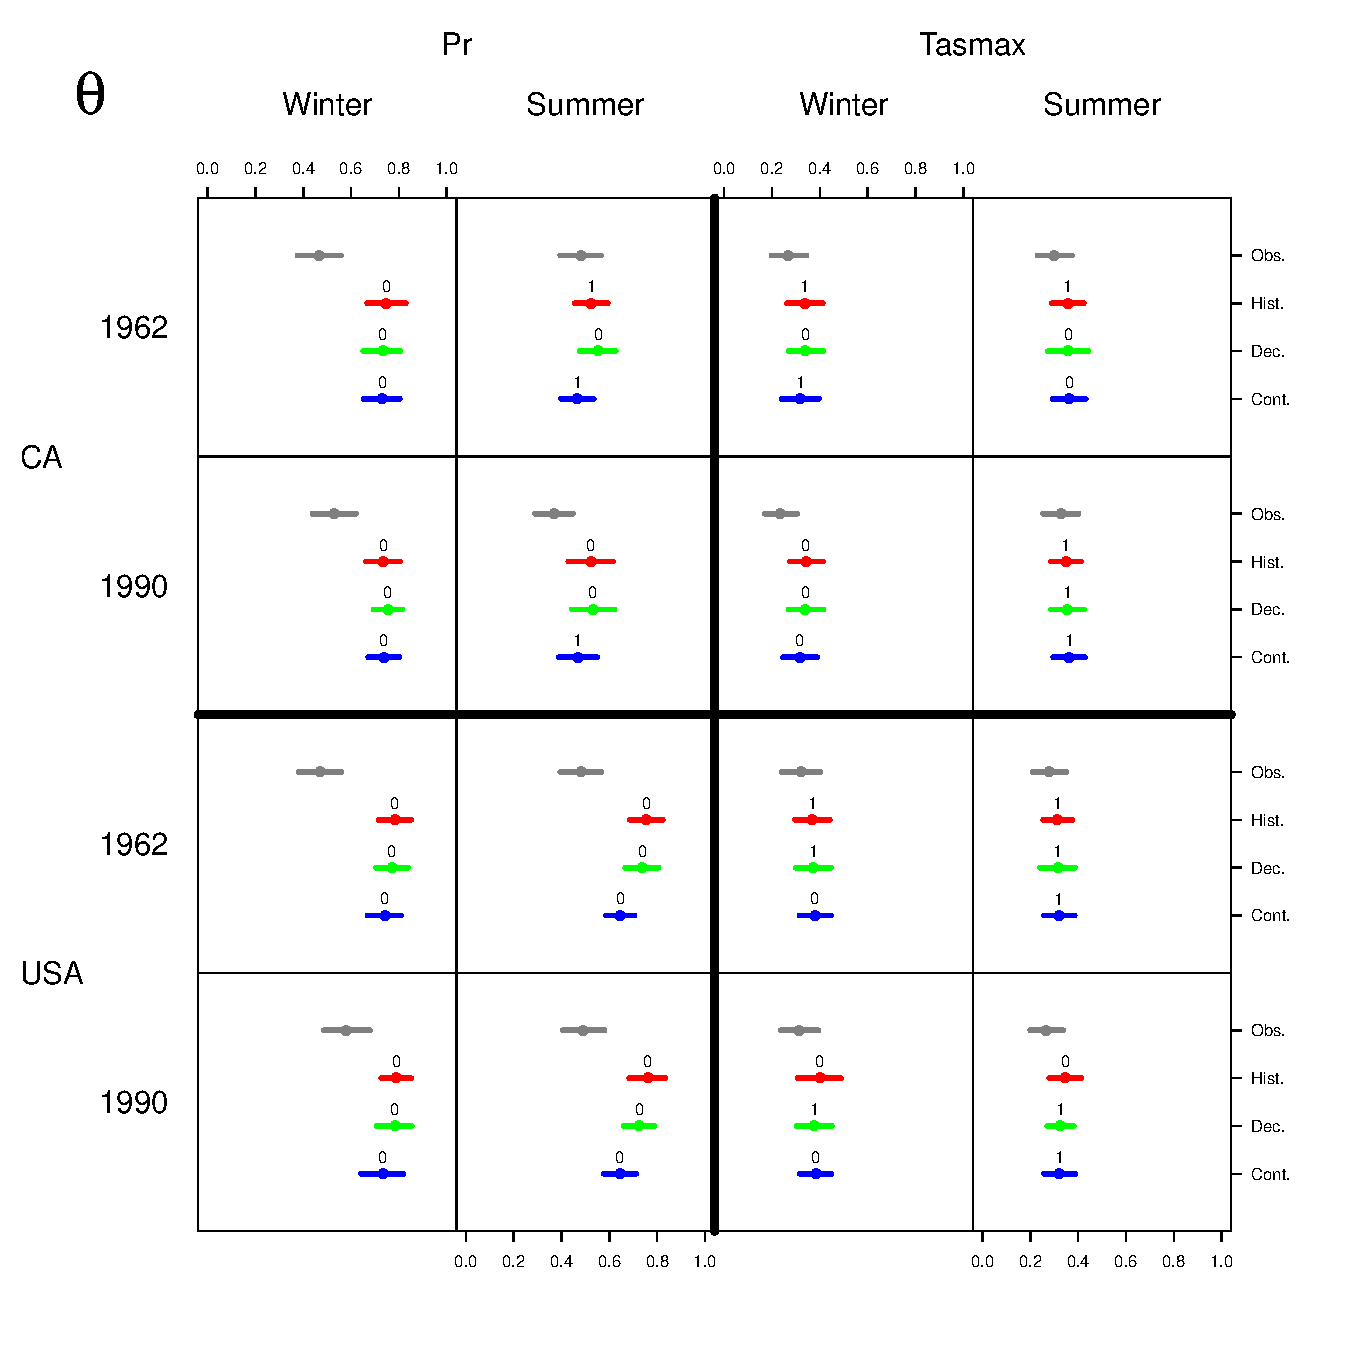
\includegraphics[scale=0.72]{figs/theta.pdf}
\end{center}
\caption{The mean extremal index. Like the parameters shown in Figures \ref{ksi} and \ref{sigma}, the hierarchical mean is shown for the CanCM4 simulations.}
\label{theta}
\end{figure}



% \section{Discussion}
% \label{discussion}
% 
% We have proposed a hierarchical threshold model to account for replicates of climate simulations. The model was applied to a variety of factor combinations and compared to a univariate threshold model for observations. This can provide a quick comparison between the simulations and the observations, but a more complete model may incorporate all factors together perhaps in a hierarchical fashion.
% 
% Our results show that the CanCM4 climate model differs from the observations in some areas, but not all.




\bibliography{refs}
\bibliographystyle{asa}

\end{document}
